\begin{frame}
\begin{itemize}
    \item What are Normalizing Flows
    \item NICE
    \item RealNVP
    \item GLOW
    \item GamePlan
    \item \textbf{\color{red}{Results}}
\end{itemize}
\end{frame}

\begin{frame}{Results: Nice Implementation}
    \begin{figure}[htbp!]
     \centering
     \begin{subfigure}[b]{0.45\textwidth}
         \centering
         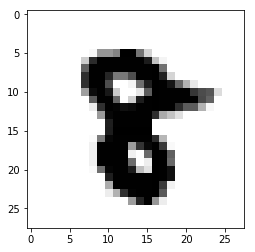
\includegraphics[width=0.5\textwidth]{Images/input.png}
         \caption{Input image}
     \end{subfigure} 
     \hfill
     \begin{subfigure}[b]{0.45\textwidth}
         \centering
         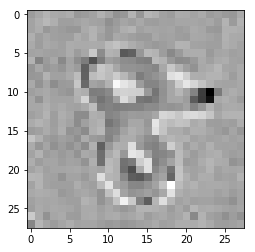
\includegraphics[width=0.5\textwidth]{Images/transformed.png}
         \caption{Transformed}
     \end{subfigure}
     \hfill
     %\caption{Forward}
\end{figure}
    \begin{figure}[htbp!]
     \centering
     \begin{subfigure}[b]{0.45\textwidth}
         \centering
         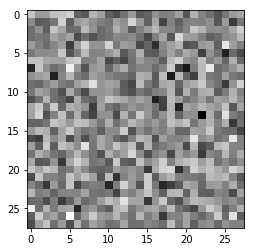
\includegraphics[width=0.5\textwidth]{Images/sample.png}
         \caption{Sample from prior}
     \end{subfigure} 
     \hfill
     \begin{subfigure}[b]{0.45\textwidth}
         \centering
         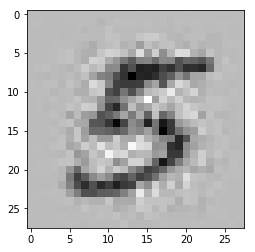
\includegraphics[width=0.5\textwidth]{Images/generated.png}
         \caption{Generated image}
     \end{subfigure}
     \hfill
     %\caption{Inverse}
\end{figure}
\end{frame}

\begin{frame}{Results: Nice Implementation}
    \begin{figure}[htbp!]
     \centering
     \begin{subfigure}[b]{0.3\textwidth}
         \centering
         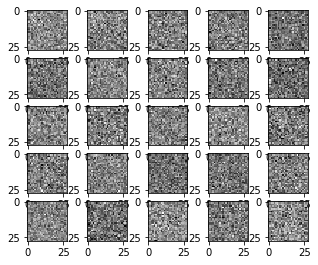
\includegraphics[width=\textwidth]{Images/prior1.png}
         %\caption{Sampled vectors}
     \end{subfigure} 
     \hfill
     \begin{subfigure}[b]{0.3\textwidth}
         \centering
         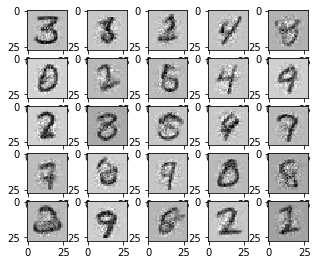
\includegraphics[width=\textwidth]{Images/mnist1.png}
         %\caption{MNIST}
     \end{subfigure}
     \hfill
     \begin{subfigure}[b]{0.3\textwidth}
         \centering
         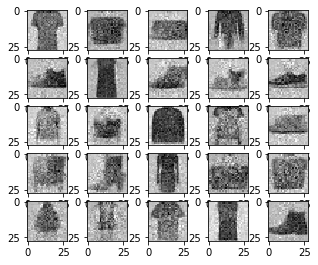
\includegraphics[width=\textwidth]{Images/fashion1.png}
         %\caption{FashionMNIST}
     \end{subfigure}
     \hfill
     \\
     \begin{subfigure}[b]{0.3\textwidth}
         \centering
         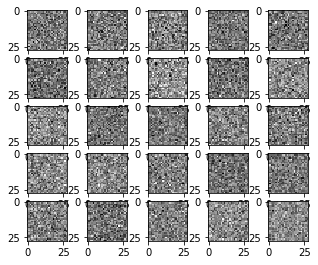
\includegraphics[width=\textwidth]{Images/prior2.png}
         \caption{Sampled vectors}
     \end{subfigure} 
     \hfill
     \begin{subfigure}[b]{0.3\textwidth}
         \centering
         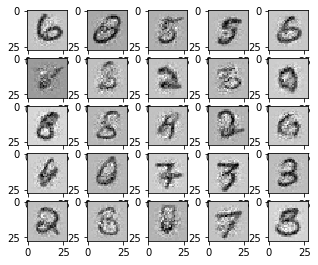
\includegraphics[width=\textwidth]{Images/mnist2.png}
         \caption{MNIST}
     \end{subfigure}
     \hfill
     \begin{subfigure}[b]{0.3\textwidth}
         \centering
         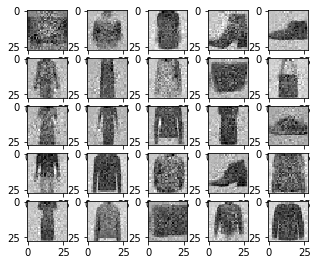
\includegraphics[width=\textwidth]{Images/fashion2.png}
         \caption{FashionMNIST}
     \end{subfigure}
\end{figure}
\end{frame}

\begin{frame}{Results: GLOW Implementation}
    \begin{figure}
        \centering
        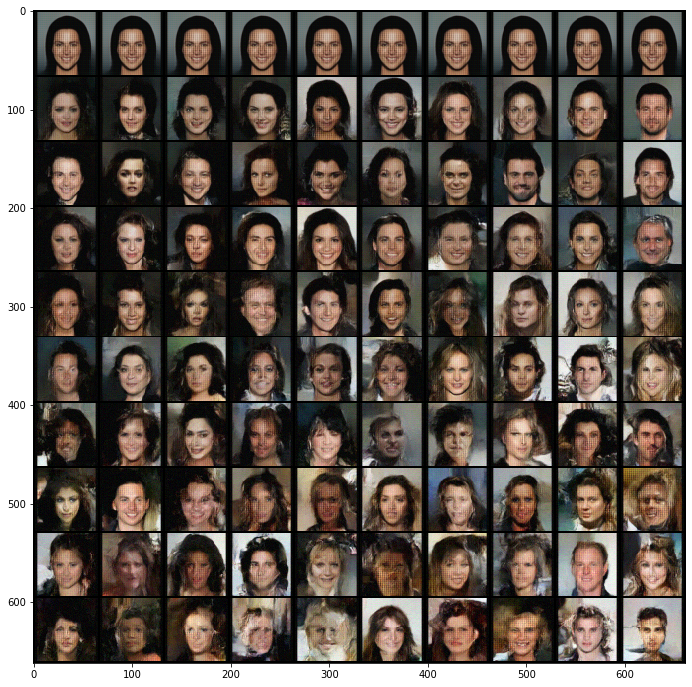
\includegraphics[width=0.8\textwidth]{Images/celeb_multiple_stds2.png}
        \caption{Caption}
    \end{figure}
\end{frame}

\begin{frame}{Results: GLOW Implementation}
    \begin{figure}[htbp!]
     \centering
     \begin{subfigure}[b]{0.3\textwidth}
         \centering
         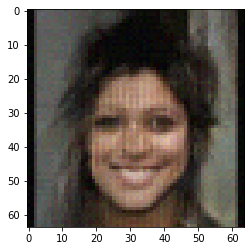
\includegraphics[width=\textwidth]{Images/celeb_sample.png}
         %\caption{Sampled vectors}
     \end{subfigure} 
     \hfill
     \begin{subfigure}[b]{0.3\textwidth}
         \centering
         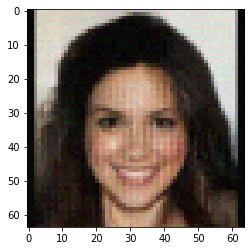
\includegraphics[width=\textwidth]{Images/celeb_sample2.png}
         %\caption{MNIST}
     \end{subfigure}
     \hfill
     \begin{subfigure}[b]{0.3\textwidth}
         \centering
         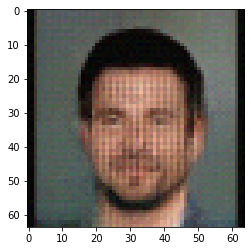
\includegraphics[width=\textwidth]{Images/celeb_sample3.png}
         %\caption{FashionMNIST}
     \end{subfigure}
     \hfill
     \caption{Images generated with GLOW}
\end{figure}
\end{frame}

\begin{frame}{Pneumonia X-ray data set}
            \begin{figure}[htbp!]
     \centering
     \begin{subfigure}[b]{0.3\textwidth}
         \centering
         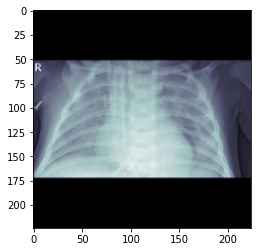
\includegraphics[width=\textwidth]{Images/xray_normal1.png}
         %\caption{Sampled vectors}
     \end{subfigure} 
     \hfill
     \begin{subfigure}[b]{0.3\textwidth}
         \centering
         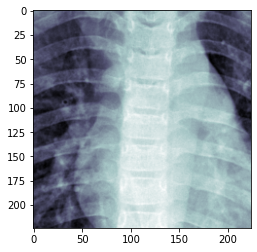
\includegraphics[width=\textwidth]{Images/xray_normal3.png}
         %\caption{MNIST}
     \end{subfigure}
     \hfill
     \begin{subfigure}[b]{0.3\textwidth}
         \centering
         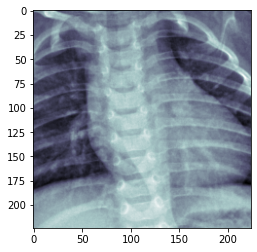
\includegraphics[width=\textwidth]{Images/xray_normal4.png}
         %\caption{FashionMNIST}
     \end{subfigure}
     \hfill
     \\
     \begin{subfigure}[b]{0.3\textwidth}
         \centering
         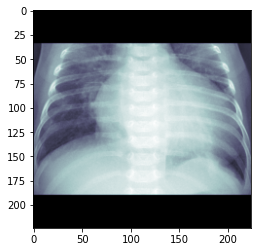
\includegraphics[width=\textwidth]{Images/xray_pneumonia1.png}
         %\caption{Sampled vectors}
     \end{subfigure} 
     \hfill
     \begin{subfigure}[b]{0.3\textwidth}
         \centering
         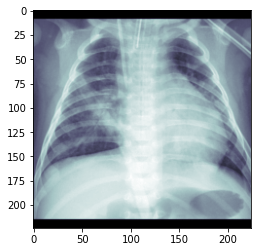
\includegraphics[width=\textwidth]{Images/xray_pneumonia2.png}
         %\caption{MNIST}
     \end{subfigure}
     \hfill
     \begin{subfigure}[b]{0.3\textwidth}
         \centering
         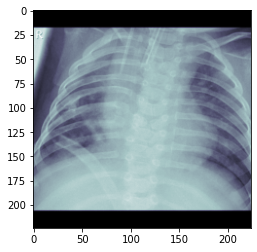
\includegraphics[width=\textwidth]{Images/xray_pneumonia5.png}
         %\caption{FashionMNIST}
     \end{subfigure}
     \caption{X-ray images: normal(top), pneumonia(bottom)}
\end{figure}
\end{frame}

\begin{frame}{Results: X-ray generation}
    \begin{figure}
        \centering
        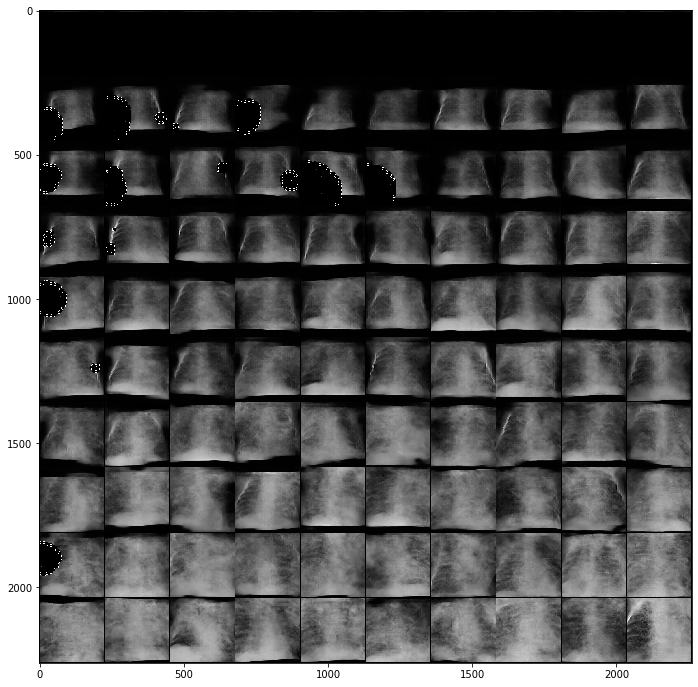
\includegraphics[width=0.8\textwidth]{Images/xray_multiple_stds.png}
        %\caption{Caption}
    \end{figure}
\end{frame}

\begin{frame}{Results: X-ray generation}
\begin{figure}[htbp!]
     \centering
     \begin{subfigure}[b]{0.3\textwidth}
         \centering
         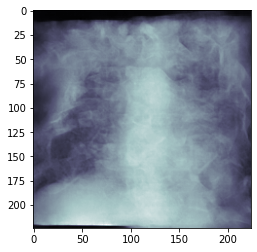
\includegraphics[width=\textwidth]{Images/xray_sample1.png}
         %\caption{Sampled vectors}
     \end{subfigure} 
     \hfill
     \begin{subfigure}[b]{0.3\textwidth}
         \centering
         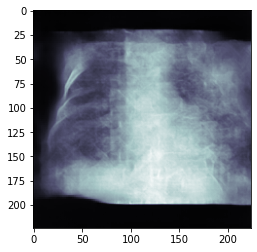
\includegraphics[width=\textwidth]{Images/xray_sample2.png}
         %\caption{MNIST}
     \end{subfigure}
     \hfill
     \begin{subfigure}[b]{0.3\textwidth}
         \centering
         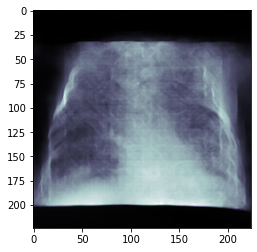
\includegraphics[width=\textwidth]{Images/xray_sample3.png}
         %\caption{FashionMNIST}
     \end{subfigure}
     \hfill
     \\
     \begin{subfigure}[b]{0.3\textwidth}
         \centering
         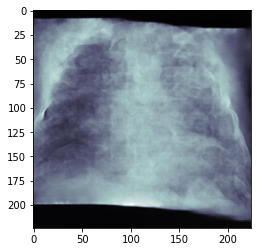
\includegraphics[width=\textwidth]{Images/xray_sample4.png}
         %\caption{Sampled vectors}
     \end{subfigure} 
     \hfill
     \begin{subfigure}[b]{0.3\textwidth}
         \centering
         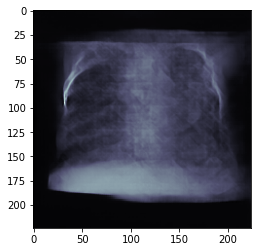
\includegraphics[width=\textwidth]{Images/xray_sample5.png}
         %\caption{MNIST}
     \end{subfigure}
     \hfill
     \begin{subfigure}[b]{0.3\textwidth}
         \centering
         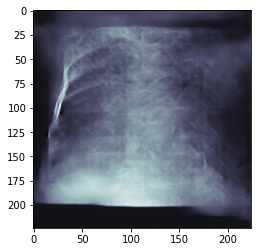
\includegraphics[width=\textwidth]{Images/xray_sample6.png}
         %\caption{FashionMNIST}
     \end{subfigure}
     \caption{Generated x-ray samples}
\end{figure}
\end{frame}

\begin{frame}{Pneumonia Classification}
    \begin{figure}
        \centering
        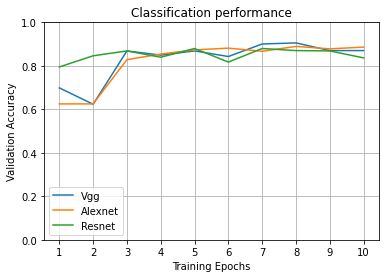
\includegraphics[width=.9\textwidth]{Images/classification_performance.png}
        %\caption{Caption}
    \end{figure}
\end{frame}

\begin{frame}{Fooling the classifiers}
    \begin{figure}
        \centering
        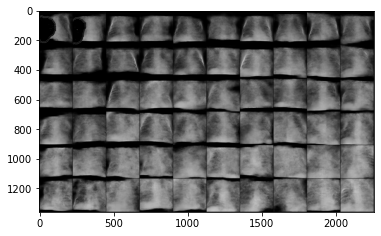
\includegraphics[width=.7\textwidth]{Images/xray_test_example.png}
        %\caption{Caption}
    \end{figure}
    \begin{itemize}
        \item Alexnet fooling accuracy: $96.667\%$
        \item Vgg fooling accuracy: $96.667\%$
        \item Resnet fooling accuracy: $0\%$
    \end{itemize}
\end{frame}

